%\documentclass{article}
%\usepackage{graphicx,subfigure}
%\begin{document}

\begin{figure}[!h]
  \centering
   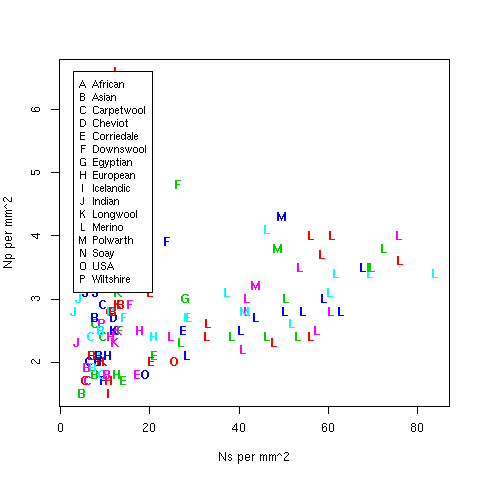
\includegraphics[width=1.0\textwidth]{NsNpalltype.png}
  \caption{Plot of breed means of secondary fibre density (Ns) and primary fibre density (Np) for 126 flocks sampled by Carter(1968)~\cite{cart:68}. The breeds have been grouped into a {\em breed type} which in some cases is an individual breed and in other cases is a country of origin. }
  \label{fig:NsNptype}
\end{figure}

%\end{document}

